\section{System Overview}
\label{sec:overview}

\begin{figure*}[t]
  \centering
  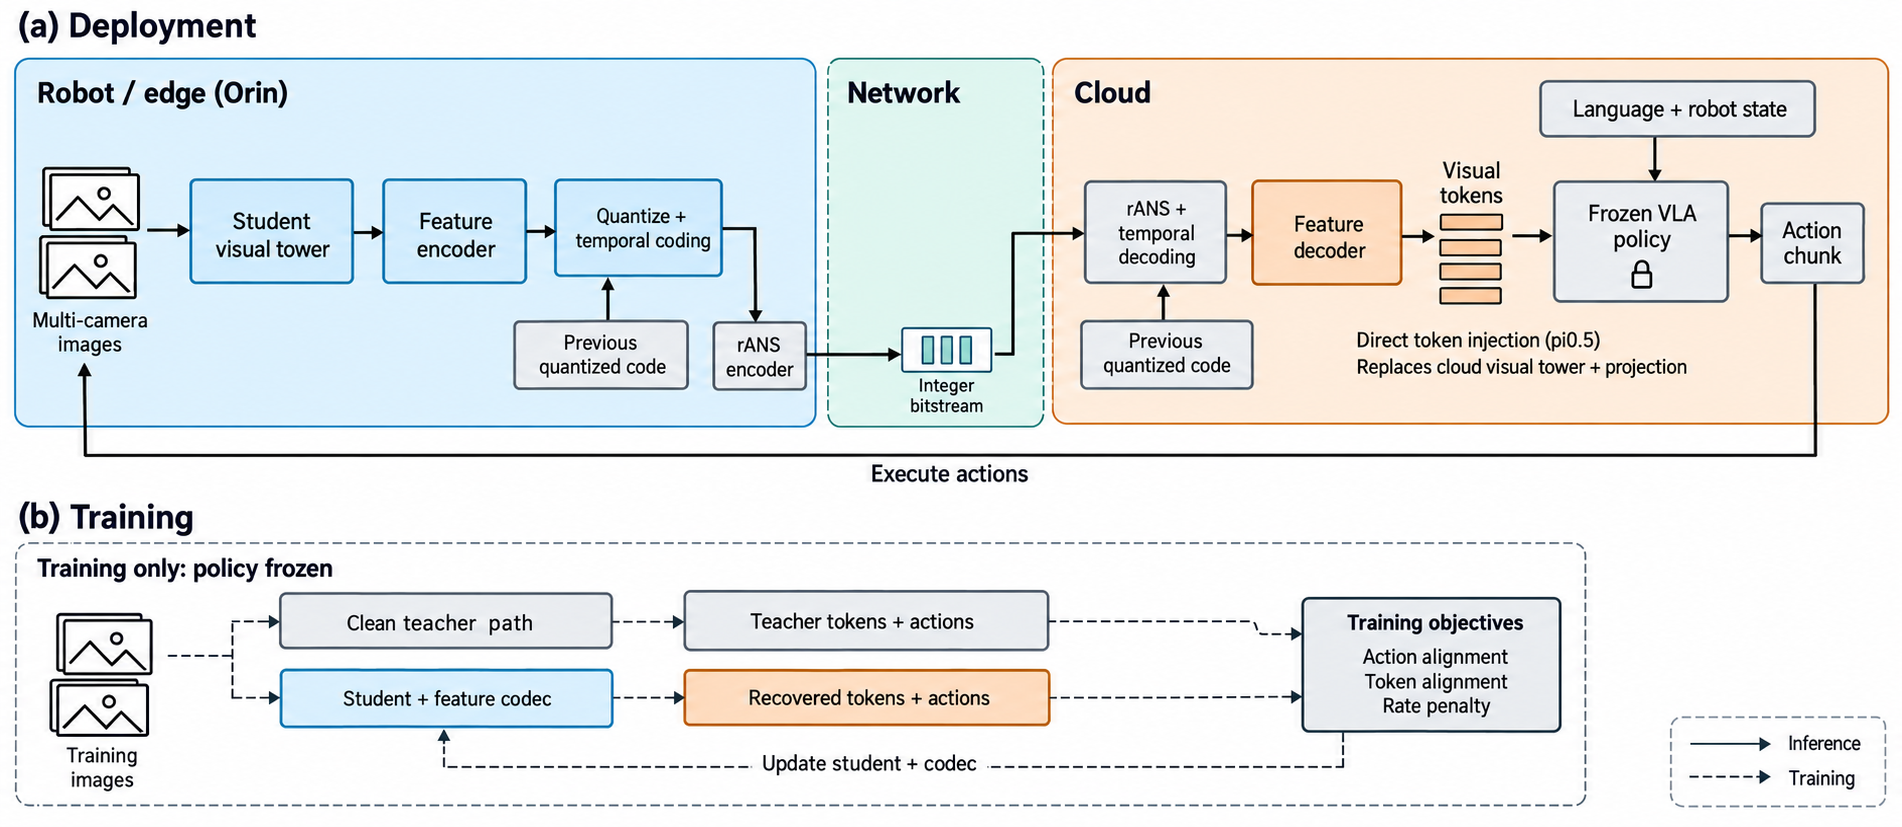
\includegraphics[width=\textwidth]{images/system-architecture-v1.png}
  \caption{System overview (primary $\pi_{0.5}$ configuration).
  (a) Deployment: the robot turns camera images into an integer bitstream;
  the cloud recovers the policy's visual tokens from the bitstream and runs
  the frozen VLA policy, skipping the cloud visual encoder.
  (b) Training: the student tower and codec are trained against the frozen
  policy's own tokens and actions on clean images, with a rate penalty.}
  \Description{Top panel: on the robot, multi-camera images pass through a
  student visual tower, feature encoder, quantization with temporal coding
  against the previous quantized code, and an rANS encoder; an integer
  bitstream crosses the network; in the cloud, rANS and temporal decoding,
  a feature decoder, and visual tokens feed a frozen VLA policy that also
  receives language and robot state and returns an action chunk. Bottom
  panel: a clean teacher path and the student-plus-codec path produce tokens
  and actions that supply action supervision, token alignment,
  and a rate penalty; only the student and codec are updated.}
  \label{fig:overview}
\end{figure*}

Each policy request incurs computation on the robot, transmission over the
network, and computation in the cloud~\cite{neurosurgeon,roboecc}.
Existing designs shift cost among the three (\S\ref{sec:bg-cost}). Image
codecs keep transmission small, but the cloud must still decode each image
and run the policy's visual encoder~\cite{limitnet,sparc}. Splitting the
policy can move that encoder onto the robot~\cite{roboecc}, where it
competes for limited compute. Our system transmits the policy's visual
features instead of images: it spends a small amount of computation on the
robot, sends a compact bitstream, and removes visual encoding from the
cloud for the primary configuration, while the policy weights stay unchanged.

\paragraph{Pipeline.}
Figure~\ref{fig:overview}a shows the deployed pipeline. On the robot, a
compact student tower distilled from the policy's visual encoder extracts
features from each camera image, and a feature encoder and quantizer map
them to integer codes. Each code is predicted from the code sent at the
previous upload, except at periodic intra frames, and the residual is
entropy-coded with integer rANS. In the cloud, the receiver reverses the
entropy and temporal coding to recover the codes exactly, and a feature
decoder turns them into visual tokens that replace the output of the
policy's visual encoder. The frozen policy consumes these tokens together
with the language instruction and robot state, which bypass the codec, and
returns an action chunk.

The design must solve four problems.

\paragraph{Preserving actions rather than appearance.}
Faithful reconstruction of images or features does not guarantee that the
policy acts the same (\S\ref{sec:bg-align}). We therefore supervise the
student tower and codec with the frozen policy's own outputs on clean
images. An action term supervises the frozen policy under recovered tokens
using clean-policy action targets, a token term aligns the tokens
themselves, and a rate term controls the coding budget
(Figure~\ref{fig:overview}b, \S\ref{sec:design-objective}).

\paragraph{Keeping robot computation small.}
Running the policy's visual encoder at every upload adds substantial
latency on resource-constrained robot hardware. The robot instead runs the
distilled student tower, trained jointly with the codec, so its work is
limited to the student tower, the feature encoder, and entropy coding
(\S\ref{sec:design-objective}).

\paragraph{Temporal coding without a decoder on the robot.}
Video codecs predict each frame from a reconstructed reference, so the
encoder also runs the decoder. For a learned codec, this would place a
neural decoder on the robot, and floating-point differences between the
robot and the cloud could desynchronize the reference. We instead predict
in the space of quantized codes, which both ends hold exactly, and use
integer-only rANS to produce identical bitstreams from the same symbols
and coding tables on ARM and x86 hosts
(\S\ref{sec:design-temporal}).

\paragraph{Adapting visual interfaces.}
Backbones consume visual features in different forms: $\pi_{0.5}$ takes
projected SigLIP tokens, whereas OpenVLA-OFT fuses features from two
visual towers. The pipeline structure is shared; the student tower and
feature decoder are adapted to each backbone's interface, and the codec is
trained once per backbone (\S\ref{sec:design-integration}).
